\chapter{BAS-RELIEF GENERATION}
Since the brush strokes are extracted individually, it is natural to independently generate the individual depth maps and then merge the depth maps together to form the desired bas-relief, see Figure \ref{decom:overview}.It is noteworthy that we use a depth map to represent a bas-relief model,which is commonly used for bas-relief generation methods.   In this Chapter, we demonstrate how to generate bas-relief from brush strokes. We also compare our algorithm against the two most notable 2D image based bas-relief generation algorithm. \\
In our implementation, we employ the orthogonal SFS \cite{prados2004unifying} algorithm on the segmented brush strokes. The brightness equation used in the SFS algorithm is expressed as,

\begin{equation*}
I(x)=\frac{1}{\sqrt{1+\lvert \bigtriangledown h \rvert ^2}}
\end{equation*}
$I(x)$ is the intensity at pixel $x$, $h(x)$ is the depth at pixel $x$. It can be noted that for higher intensity $I$, change of depth $h$ is smaller. Some brush strokes are painted by colors with high intensity. As a result, if the shape from shading algorithm is performed on intensity, the resulting stroke models will become flat and lack of hierarchy. The opacity of image is independent of the color intensity (see Figure \ref{histo}). Each stroke has an appropriate distribution of opacity, which is in favor of a layered look, so we reformulate the equation : 
\begin{equation*}
\alpha(x)=\frac{1}{\sqrt{1+\lvert \bigtriangledown h \rvert ^2}}
\end{equation*}
$\alpha(x)$ is the opacity value of pixel $x$ on a brush stroke. 
To make the bas-relief more inflated,we rewrite the as,

\begin{equation}
\lVert \bigtriangledown h \rVert = \sqrt{\frac{1}{\lVert \alpha(x) \rVert ^2}-1+ \Delta}
\end{equation}
where $\Delta$ is a positive displacement. This modification may make the surface inflated. By using fast marching algorithm \cite{sethian1999level} to solve this equation, we can generate a depth map for each brush stroke. As show in Figure \ref{strokerelief}, we input the opacity map of a decomposed layer, and from that layer we extract three brush strokes shown in different color. Then by applying our algorithm we can generate bas-reliefs(depth maps) from each one of the brush strokes on this layers.By generating depth map from all brush strokes,and merge them together, we automatically output a bas-relief from the input Chinese painting. \\
To differentiate the bas-relief generated form a single stroke and the bas-relief generated from the whole painting, we use the term "stroke-relief" to indicate a bas-relief(depth map) generated from a single stroke. And just like a Chinese painting can be regarded as a union of brush strokes \cite{xu2006animating} ,in our approach, a bas-relief can be regarded as a union of stroke-relief.Since the stroke-reliefs are independent of each other, the order and shape may be redefined by the users. It is suitable for further editing in bas-relief design.
\begin{figure}[H]
	\centering
	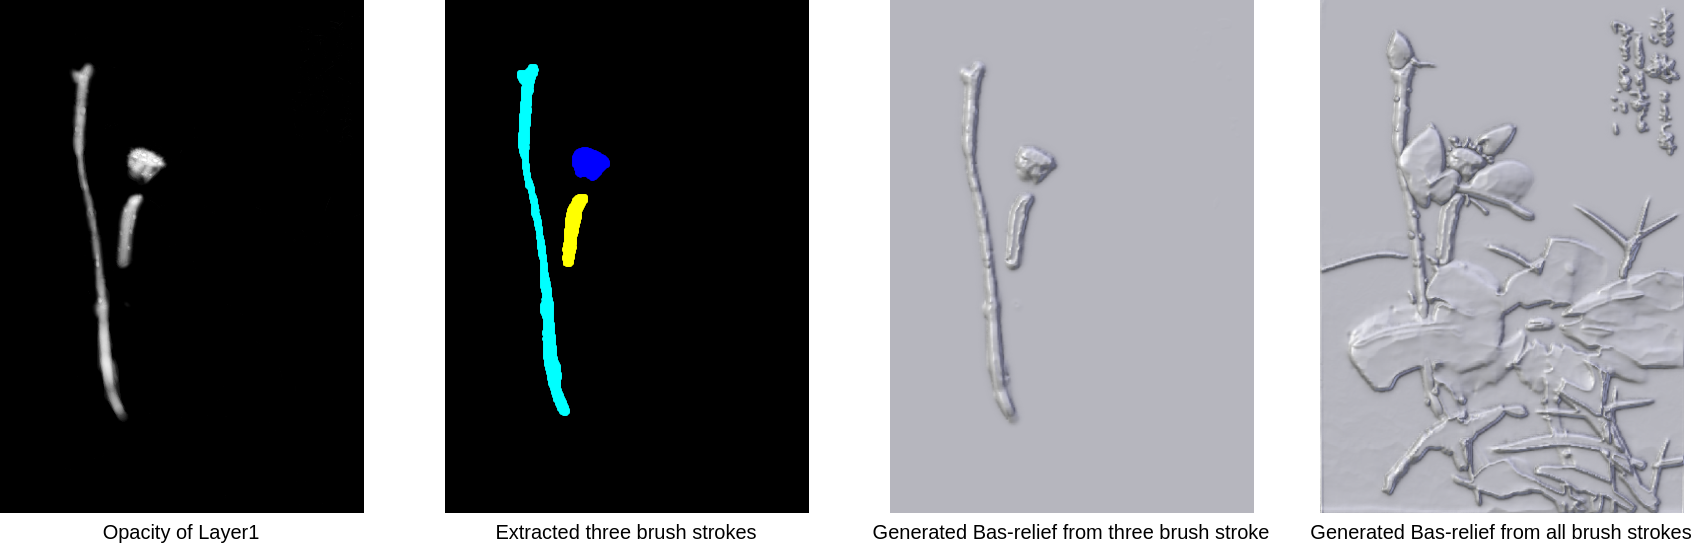
\includegraphics[width=15cm]{strokerelief.png}
	\caption{Bas-relief generation from brush strokes}
	\label{strokerelief}
\end{figure}

Figure \ref{ch1} and Figures in section \ref{more results} show our bas-relief results generated for various Chinese paintings. 

\begin{figure}[H]
	\centering
	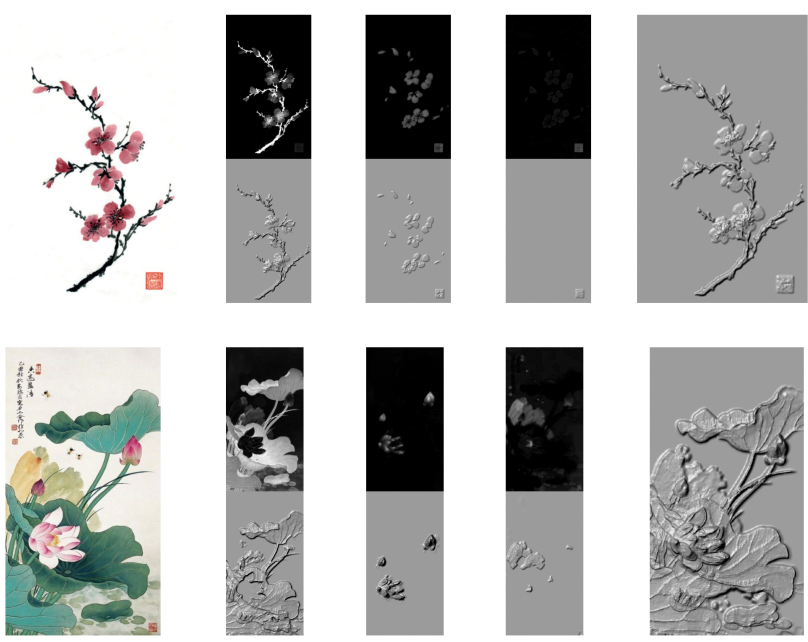
\includegraphics[width=15cm]{rose1.png}
	\caption{Bas-relief generation from Chinese paintings}
\end{figure}\label{ch1}

\section{Comparisons of Bas-relief Generation}\label{compare}
Most of other 2D images based methods is unsuited for our aim due to some simply reasons, which is explained in section \ref{2dimagebased} and section \ref{ref2dimage}.\\
Since our generation is based on opacity of brush strokes and each stroke occupies a 2D region on canvas,in this section, we compares our bas-relief generation method against another alternative notable 2D image based bas-relief generation method \cite{zeng2014region}. \\
Zeng et al.'s work \cite{zeng2014region} present region-based algorithm for bas-relief generation.At first,their method segments input image into 2D regions and determines the layer of the regions. Then, they reconstruct relief from each layer. And they demonstrate this algorithm works well for a range of input photos, including human faces, flowers and animals.\\
In their method, to extract regions from the image, the feature lines are detected at first. Next, seed points are derived from these lines, and regions are found from them using a region growing process. The region extraction in their method is quite similar with our brush stroke extraction process. For Chinese painting, a brush stroke can be considered as a region on canvas. So we compare our method against Zeng et al.'s method \cite{zeng2014region} based on three factors mentioned in Section \ref{2dimagebased} : depth information, silhouettes and edges,fine details. \\
\textbf{Depth information:} In the Zeng et al.'s work \cite{zeng2014region} , regions determine the depth information, so regions have to be faithfully extracted. The first step of extract regions is detect region outlines by line detection on intensity map. Naturally, the line detection fails in following scenarios: \\
(1) The brush stroke with the intensity very close to the background; \\
(2) Two adjacent brush stroke painted by different colors with the similar intensity;\\
So, their algorithm would fail at the first step.\\
In our algorithm, the above mentioned problems is avoided by layer decomposition and stroke extraction , see Section \ref{extract}. By extracting brush stroke faithfully, we follow the manner of Chinese painting, generate bas-relief from all brush strokes. \\
\textbf{Silhouettes and Edges:} As mention above, the region-based algorithm fails to find the outlines of brush strokes, namely, it can not separate brush strokes from the background or generate a reasonable contrast between the foreground objects and the background as a starting establishment for interpreting heights. On the other hand, since our method apply layer decomposition at first, foreground(brush strokes) is easily separated from background. \\
\textbf{Fine Details:} Region-based algorithm performs shape from shading on the intensity of the image.As we mentioned,for brush strokes painted by bright color, the generated bas-relief would be flat and features can not be well preserved. In our algorithm, we use opacity to generate the bas-relief, which maintains the details of brush strokes better, see Figure \ref{histo}.  \\

 